\begin{frame}{Qudrilateral}
{\textbf{Problem:5}\\Construct a kite EASY if AY = 8, EY = 4 and SY = 6.}
\begin{itemize}
\item \textbf{Solution:}
\end{itemize}
\textbf{Given:}\\
AY = 8cm, EY = 6cm, SY = 7cm.\\
from the Quadrilaterel EASY\\
we know the upper two sides and lower two sides of a kite is equal\\ 
i.e EA = EY = 6cm and SA = SY = 7cm.\\

the python code for  Figure 0-9 is /codes/quad\_con.py\\
and the equivalent latex-tikz for Figure 0-10 is /figs/quad\_con.tex
\end{frame}
\begin{frame}
\textbf{Construction Of Quadrilateral:}\\
Consider the $\Delta$ AOE
\begin{align}
AE^2 = AO^2 + OE^2
\end{align}
$6^2 = 4^2$ + OE$^2$\\
OE = $\sqrt{20}$.\\
From the $\Delta$ AOS
\begin{align}
YS^2 = YO^2 + OS^2
\end{align}
$7^2 = 4^2$ + OS$^2$\\
OS = $\sqrt{33}.$\\
\end{frame}
\begin{frame}{}
\begin{figure}[!ht]
	\begin{center}
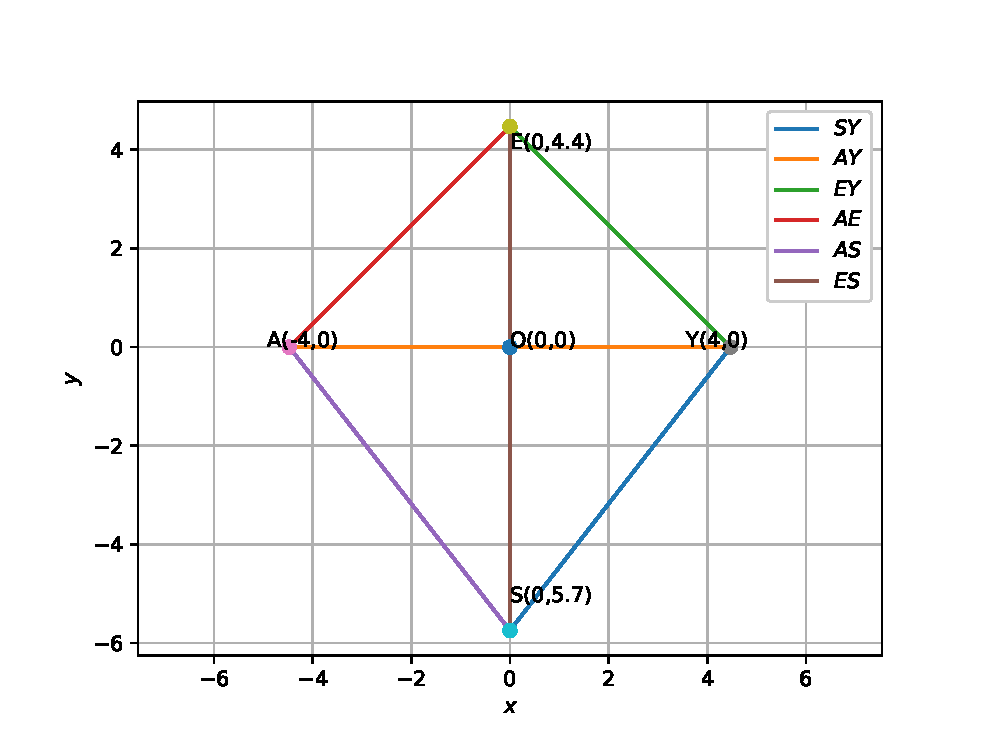
\includegraphics[width=0.8\columnwidth]{./figs/quad_con.eps}
	\end{center}
	\caption{Quadrilateral}
	\label{}	
\end{figure}
\end{frame}
\begin{frame}{}
\begin{figure}[!ht]
	\begin{center}
		\resizebox{0.6\columnwidth}{!}{\begin{tikzpicture}
[scale=0.5,>=stealth,point/.style={draw,circle,fill = black,inner sep=0.5pt},]

%quadrilateral sides
\def\a{4.4}
\def\b{5.7}
\def\c{4}

%Labeling points
\node (E) at (0,\a)[point,label=above:$E$] {};
\node (A) at (-\c,0)[point,label=left:$A$] {};
\node (S) at (0,-\b)[point,label=below:$S$] {};
\node (Y) at (\c,0)[point,label=right:$Y$] {};
\node (O) at ($(A)!0.5!(Y)$)[point,label=right:$O$] {};
%Drawing Quadrilateral EASY
\color{blue}
\draw (E)--node[above] {$\textrm{6}$}(A)--node[left] {$\textrm{7}$}(S)--node[right] {$\textrm{}$}(Y)--node[right] {$\textrm{}$}(E)--node[right] {$\textrm{}$}(S)(A)--node[below left]{$\textrm{4}$}(O)--node[left]{$\textrm{}$}(Y)(O)--node[right]{$\textrm{$\sqrt{20}$}$}(E)(O)--node[right]{$\textrm{$\sqrt{33}$}$}(S);

%Drawing and marking angles
\color{black}
\tkzMarkAngle[fill=black!40,size=0.8cm,mark=](O,A,E)
\tkzMarkAngle[fill=black!40,size=0.8cm,mark=](S,A,O)
\tkzMarkRightAngle[fill=blue!20,size=.3](A,O,E)
\tkzMarkRightAngle[fill=blue!20,size=.3](Y,O,E)
\tkzMarkRightAngle[fill=blue!20,size=.3](A,O,S)
\tkzMarkRightAngle[fill=blue!20,size=.3](Y,O,S)
\end{tikzpicture}
}
	\end{center}
	\caption{Quadrilateral}
	\label{}	
\end{figure}
\end{frame}
\begin{frame}
\textbf{Coordinates of quadrilateral:}
\\
Construct a quadrilateral(Kite) EASY\\
\begin{enumerate}
\item A =$\begin{pmatrix} -4\\0 \end{pmatrix}$ and Y is $\begin{pmatrix}  4\\0 \end{pmatrix}$
\item O is taken as the origine i.e at $\begin{pmatrix} 0\\0 \end{pmatrix}$
\item The coordinates of E and S are  $\begin{pmatrix}  0\\ \sqrt{20} \end{pmatrix}$ $\begin{pmatrix} 0\\-\sqrt{33} \end{pmatrix}.$
\end{enumerate}
\url{https://github.com/Narendrapulipati/geometry/blob/master/codes/quad_con.py}
\url{https://github.com/Narendrapulipati/geometry/blob/master/figs/quad_con.tex}
\end{frame}